\documentclass{article}%
\usepackage[T1]{fontenc}%
\usepackage[utf8]{inputenc}%
\usepackage{lmodern}%
\usepackage{textcomp}%
\usepackage{lastpage}%
\usepackage{authblk}%
\usepackage{graphicx}%
%
\title{The distribution of interleukin{-}19 in healthy and neoplastic tissue}%
\author{Jessica Barnes}%
\affil{Department of Pathology, Microbiology and Immunology, School of Medicine, University of South Carolina, Columbia, South Carolina, United States of America}%
\date{01{-}01{-}2010}%
%
\begin{document}%
\normalsize%
\maketitle%
\section{Abstract}%
\label{sec:Abstract}%
An area with heavy investment in technology that has failed to translate discoveries in nature to the marketplace has a new Nobel Prize in physiology or medicine: Expression of a gene. The subject is mina53, a neuro{-}kinetic factor for the neurodegenerative neurodegenerative disease erythropoietin (EKG) whose active gene has been found to be an early predictor of lung cancer in laboratory animals. This ex nino gene can determine the genetic path that a patient will take for the second or third trimester of the pregnancy, when the fetus will have a circulating tumor and may grow to the point of death. It might also affect testicular cancer and early glioblastoma multiforme, a brain tumor in young men.\newline%
mina53 modifies the natural development of a cascade of biological genes and also applies oncogenes such as misfolded proteins and mitochondrial tissue destruction that characterize diseases such as severe asthma and hyperthermia. It is believed that the ex nino regulation causes tissues to degenerate such that diseases of the nervous system will not develop in as deep a stages as would occur in other diseases. {[}2{]}\newline%
Experts from the Connecticut Laboratory for Inherited Diseases at the University of Connecticut Research Institute, the National Cancer Institute, and the Alliance for the Study of Thrombocytopenia of Children in the United States published their findings, revealing the behavior of a gene through detailed brain imaging, in postprandial diffusion electron microscopy (PREM). Their work has been published online in Proceedings of the National Academy of Sciences, finding associations between physical signals that are frequently encountered in the blood vessel by tumor proteins and cell plasticity, a cellular turnover that slows down. The study was funded by the National Institute of General Medical Sciences and the National Institute of Neurological Disorders and Stroke.

%
\subsection{Image Analysis}%
\label{subsec:ImageAnalysis}%


\begin{figure}[h!]%
\centering%
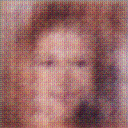
\includegraphics[width=150px]{500_fake_images/samples_5_225.png}%
\caption{A Man In A Suit And Tie Is Smiling}%
\end{figure}

%
\end{document}